\documentclass[11pt,reqno,final]{amsart}

\pdfcompresslevel=0
\pdfobjcompresslevel=0

\usepackage[dvipsnames]{xcolor}% adds colors
\usepackage{amsmath, amsthm}% {amsfonts, amssymb}

% New Characters
\usepackage[latin1]{inputenc}%
\usepackage[T1]{fontenc}

\usepackage{MnSymbol}
\usepackage[normalem]{ulem}% underlining

\usepackage[theoremfont, largesc]{newpxtext} % different text,math font
\usepackage{newpxmath}

\makeatletter
\DeclareMathRadical{\sqrtsign}{symbols}{112}{largesymbols}{112}
% \let\sqrt=\undefined
% \DeclareRobustCommand\sqrt{\@ifnextchar[\@sqrt{\mathpalette\@x@sqrt}]}
% \def\@x@sqrt#1#2{%
%  \setbox\z@\hbox{$\m@th#1\sqrtsign{\mkern1mu #2}$}
%  \mkern3mu\box\z@}
\makeatother




% Page Typesetting
\usepackage[final]{microtype}
\usepackage{relsize}
\usepackage[margin=1in]{geometry}
\usepackage{framed}
\usepackage{tikz}
\usepackage{setspace}

\usepackage{hyperref}
\hypersetup{
  final,
  pdftitle={Math 135 - Project 2},
  pdfauthor={Bonventre}, 
  linktoc=page,
  pagebackref,
  colorlinks=true,
  citecolor=PineGreen,
  linkcolor=PineGreen,
  linkbordercolor=PineGreen,
}


% Internal References

\usepackage[inline,shortlabels]{enumitem}

\numberwithin{equation}{section} 
\numberwithin{figure}{section}

\usepackage[nameinlink,capitalise,noabbrev]{cleveref}

\crefname{equation}{}{} % get \cref to behave as \eqref

% \theoremstyle{plain} % bold name, italic text
\newtheorem{theorem}[equation]{Theorem}%
\newtheorem*{theorem*}{Theorem}%
\newtheorem{lemma}[equation]{Lemma}%
\newtheorem{proposition}[equation]{Proposition}%
\newtheorem{corollary}[equation]{Corollary}%
\newtheorem{conjecture}[equation]{Conjecture}%
\newtheorem*{conjecture*}{Conjecture}%
\newtheorem{claim}[equation]{Claim}%


\theoremstyle{definition} % bold name, plain text
\newtheorem{definition}[equation]{Definition}%
\newtheorem*{definition*}{Definition}%
\newtheorem{example}[equation]{Example}%
\newtheorem*{example*}{Example}%
\newtheorem{remark}[equation]{Remark}%
\newtheorem{notation}[equation]{Notation}%
\newtheorem{convention}[equation]{Convention}%
\newtheorem{assumption}[equation]{Assumption}%
\newtheorem{exercise}{Exercise}
\newtheorem{question}{Problem}

% ---------- macros
\newcommand{\set}[1]{\left\{#1\right\}}%
\newcommand{\sets}[2]{\left\{ #1 \;|\; #2\right\}}%
\newcommand{\longto}{\longrightarrow}%
\newcommand{\into}{\hookrightarrow}%
\newcommand{\onto}{\twoheadrightarrow}%

\usepackage{harpoon}
\newcommand{\vect}[1]{\text{\overrightharp{\ensuremath{#1}}}}

\newcommand{\del}{\partial}%

\newcommand{\ki}{\chi}
\newcommand{\ksi}{\xi}
\newcommand{\Ksi}{\Xi}

\newcommand{\dlim}{\displaystyle\lim}

\DeclareMathOperator{\sech}{sech}

% %%%%%%%%%%%%%%%%%%%%%%%%%%%%%%%%%%%%%%%%%%%%%%%%%%%%%%%%%%%%%%%%%%%%%%%%%%%%%%%%%%%%%%%%%%%%%%%%%%%%

\begin{document}
\onehalfspacing

\begin{center}
        \textbf{\Large Math 135, Calculus 1, Fall 2020}\\[10pt]
        {\large Project 2: Hyperbolic Functions.}\\
        Due: \textbf{Friday, October 30} by 11:59pm.
\end{center}

\thispagestyle{empty}

\renewcommand{\thesection}{\Alph{section}}


\section*{The Project}

In this project, you will investigate a new family of functions called \textbf{hyperbolic functions}.
These are analogues of the ordinary trigonometric functions
based on the ``unit byperbola $x^2 - y^2 = 1$ as opposed to the unit circle:
\begin{center}
        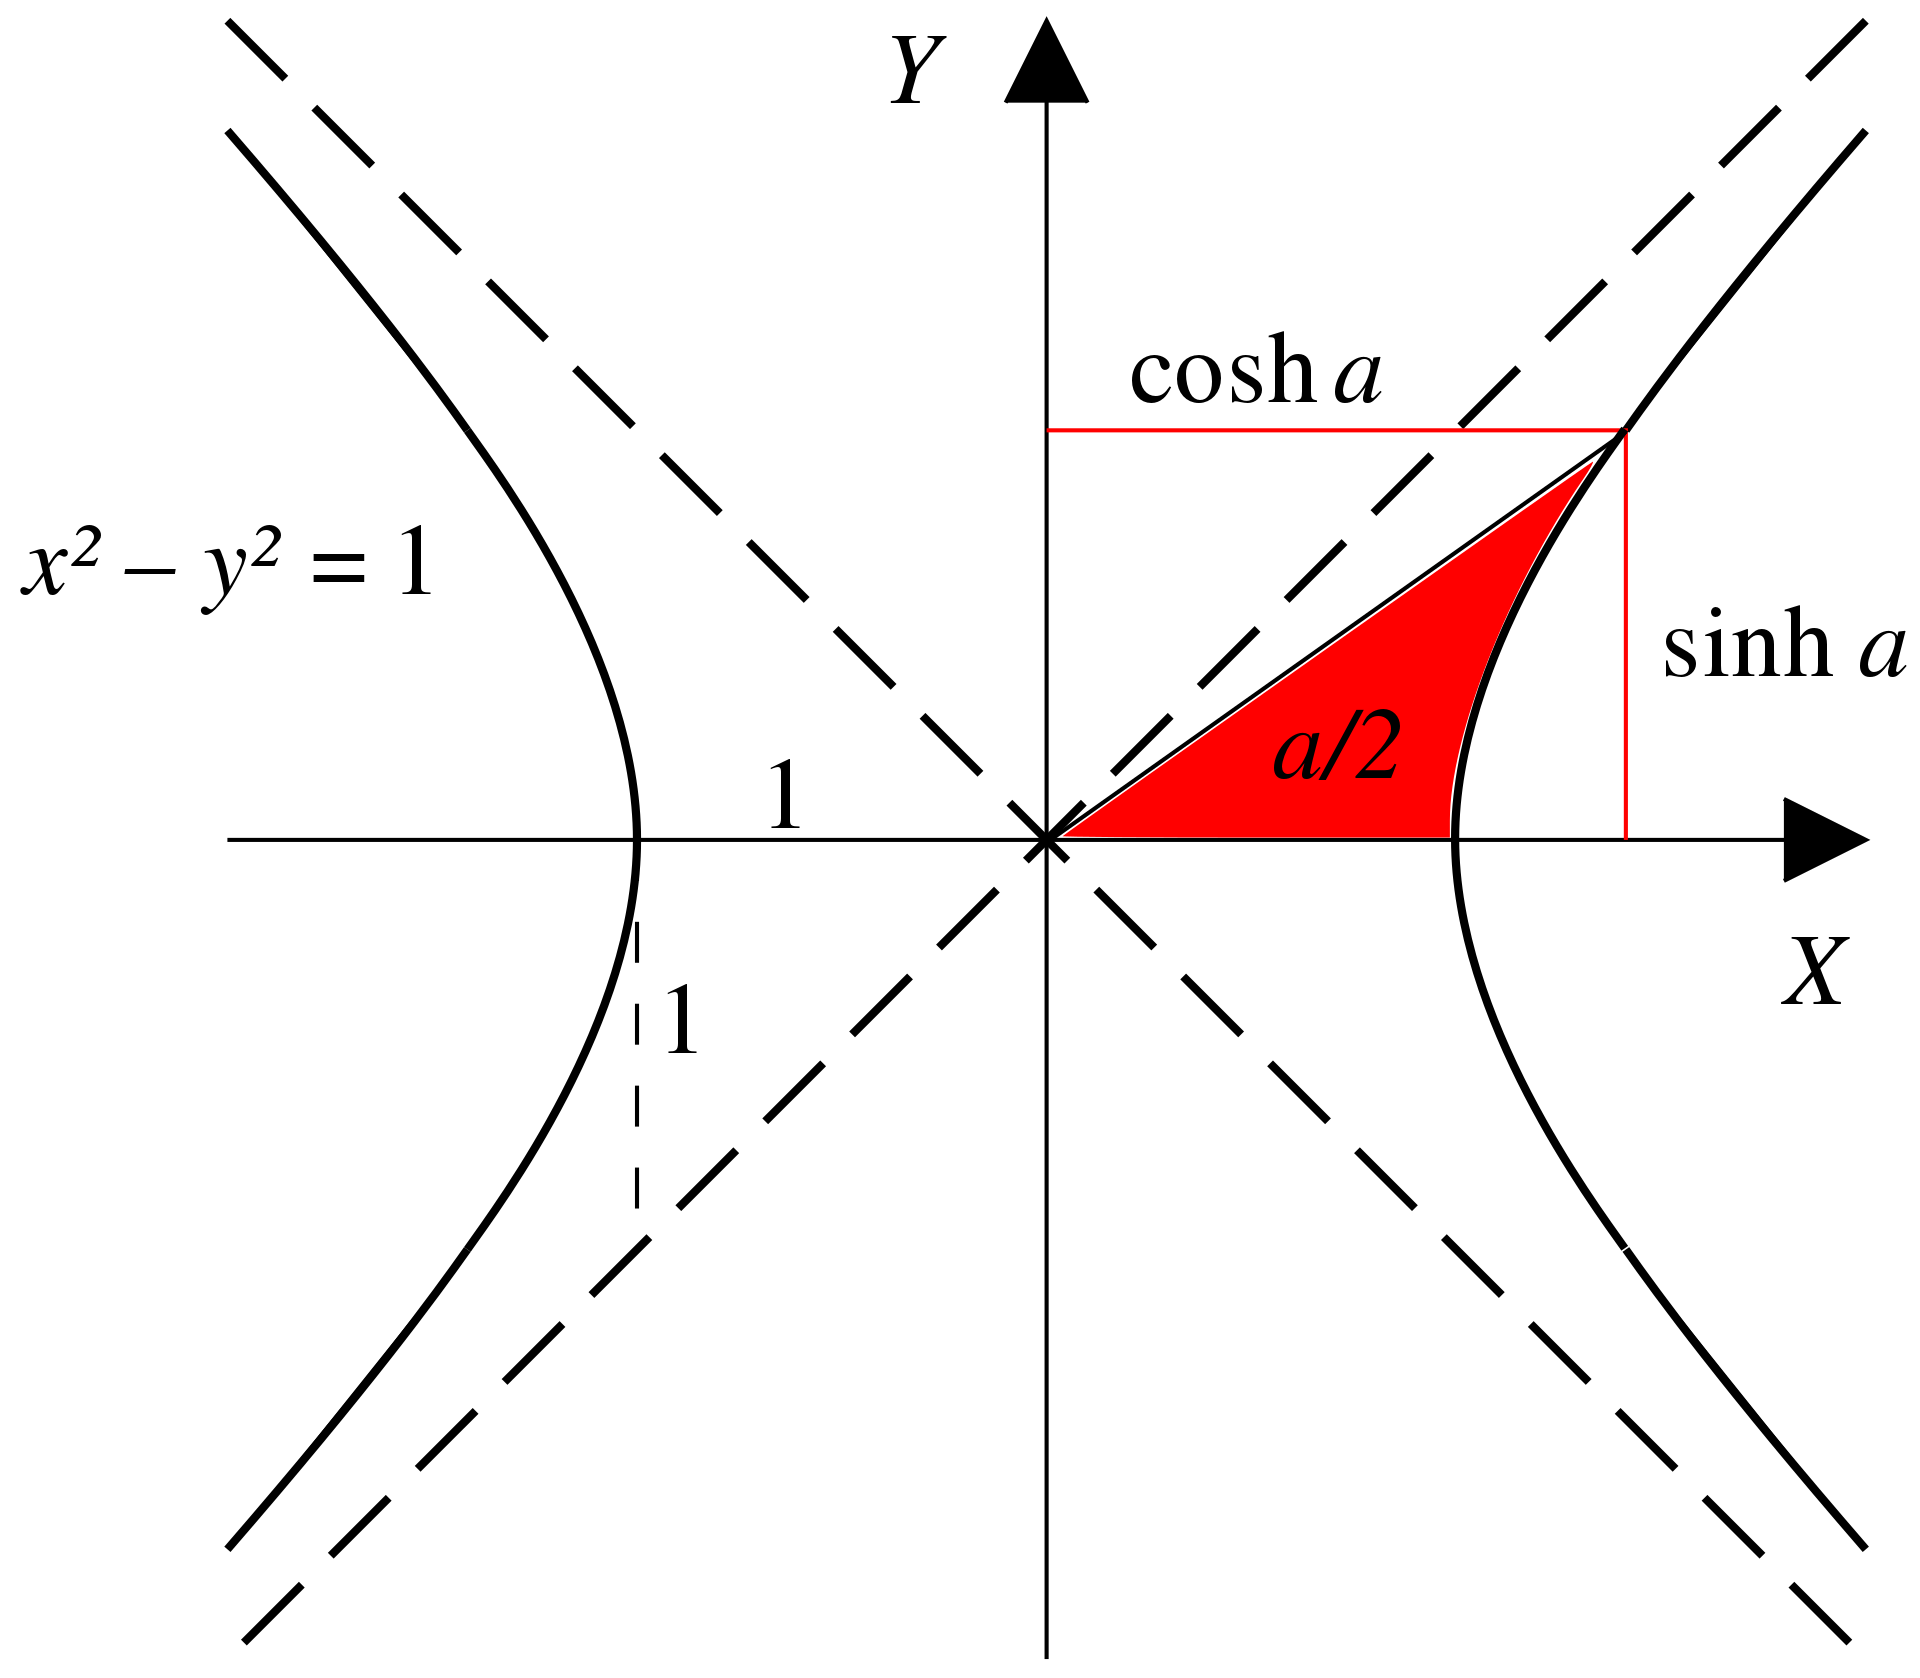
\includegraphics[width=2.5in]{hyp.png}
\end{center}

\subsection*{Components}

This project will consist of a single document, your report.
This will include the answer to a variety of questions, as well as several graphs and visual analyses.

\subsection*{Setup}

There are explicit formula, in terms of the exponential function $e^x$, for the basic hyperbolic functions:
\begin{itemize}
\item \textbf{hyperbolic sine} is defined to be
        \[
                \sinh t = \dfrac{e^t - e^{-t}}{2}.
        \]
\item \textbf{hyperbolic cosine} is defined to be
        \[
                \cosh t = \dfrac{e^t + e^{-t}}{2}.
        \]
\item \textbf{hyperbolic tangent} is defined to be
        \[
                \tanh t = \dfrac{\sinh t}{\cosh t}.
        \]
\item \textbf{hyperbolic secant} is defined to be
        \[
                \sech t = \dfrac{1}{\cosh t}.
        \]        
\end{itemize}

\newpage


\section{Graphs of hyperbolic functions}

We begin by investigating the graphs of these functions.

\begin{question}
        $ $
        \begin{enumerate}[(a)]
        \item Graph the four hyperbolic functions above, and include these in your report.
        \item Based on these graphs, what is the domain and range of each of these functions?
        \item Confirm your answer for the \textbf{domains} using algebra.
                How does this relate to the analogous trig functions?
        \end{enumerate}
\end{question}

\begin{question}
        $ $
        \begin{enumerate}[(a)]
        \item Based on these graphs, what are the horizontal asymptotes for $\tanh t$? Confirm your answer using algebra.
        \item Graph $\tanh t$ and $\arctan t$ on the same set of axes, and include this in your report.
                What similarlities do you notice?
        \end{enumerate}
\end{question}

\begin{question}
        $ $
        \begin{enumerate}[(a)]
        \item Based on these graphs, for each of these four hyperbolic functions, decide if the function is: even, odd, or neither.
        \item Using algebra and the definition of even and odd functions, prove your assertions from Part 3a.
        \end{enumerate}
\end{question}

\begin{question}
        $ $
        \begin{enumerate}[(a)]
        \item On \url{desmos.com/calculator}, draw $(\cosh t, \sinh t)$ for $-2 \leq t \leq 2$.
                Include this in your report.
        \item Using the explicit definitions from the introduction, show the identity $\cosh^2 t - \sinh^2 t = 1$,
                confirming that $(\cosh(t),\sinh(t))$ lie on the unit hyperbola $x^2 - y^2 = 1$.
        \end{enumerate}
\end{question}
\vfill

\section{Calculus of hyperbolic functions}

        The derivative formulas for the hyperbolic functions are very similar (but not identical) to those for the trigonometric functions:

\begin{question}
        Show that $\dfrac{d}{dt}\Big( \sinh t \Big) = \cosh t$.
\end{question}

\begin{question}
        $ $
        \begin{enumerate}[(a)]                
        \item Find formula for $\dfrac{d}{dt}\Big( \cosh t \Big)$ and $\dfrac{d}{dt}\Big( \tanh t \Big)$ in terms of other hyperbolic functions.
                Show all work that led to these formulas.
        \item What simple second-order differential equation is $y = \sinh t$ a solution?\\
                (\textit{Hint: see Written HW 10-23, Exercise 1.})
        \end{enumerate}
\end{question}

\vfill

\newpage

\section{Inverses of hyperbolic functions}

We would like to compute the inverse functions for some of these hyperbolic functions.

\begin{question}
        Use the explicit definition from the introduction to find the exact value of $t$ such that $\sinh t = \dfrac{3}{4}$.\\
        (\textit{Hint: Leave your answer as a logarithm.})
\end{question}

\begin{question}
        $ $
        \begin{enumerate}[(a)]
        \item Graphically, it is clear that $\sinh t$ passes the horizontal line test, and hence is 1-to-1.
                Confirm this by using calculus to show that $\sinh t$ is always increasing.
        \item Show that $\sinh^{-1}(y) = \ln(y + \sqrt{y^2+1})$.\\
                (\textit{Hint: When solving for $t$ in $\sinh t = y$, first set $e^t = z$ and solve for $z$.\\
                You will need to use the quadratic formula. Why is only \textbf{one} of the possible solutions valid?})
        % \item Show that $\tanh^{-1}(t) = \dfrac{1}{2} \ln\left( \dfrac{1+x}{1-x} \right)$.                
        \end{enumerate}
\end{question}

\begin{question}
        We will find the derivative of $\sinh^{-1}(t)$ in two different ways:
        \begin{enumerate}[(a)]
        \item Use Implicit Differentiation, as used in Worksheet 10-26 to compute $\dfrac{d}{dx}(\cos^{-1}(x))$,
                to compute the derivative of $\sinh^{-1}(t)$.
        \item Use the formula $\sinh^{-1}(t) = \ln\left(t + \sqrt{t^2+1}\right)$ and $\dfrac{d}{dt}(\ln(t)) = \frac{1}{t}$ (see Worksheet for 10-26)
                to compute the derivative of $\sinh^{-1}(t)$.
        \end{enumerate}
\end{question}







\end{document}
